\documentclass[a4paper, 12pt]{article}

\usepackage{geometry}
\geometry{a4paper,
total={170mm,257mm},left=2cm,right=2cm,
top=1cm,bottom=2cm}
\usepackage{wrapfig}
\usepackage{graphicx}
\usepackage{mathtext}
\usepackage{amsmath}
\usepackage{siunitx} % Required for alignment
\usepackage{multirow}
\usepackage{gensymb}
\usepackage{rotating}
\sisetup{
  round-mode          = places, % Rounds numbers
  round-precision     = 2, % to 2 places
}

\usepackage[T1,T2A]{fontenc}

\usepackage[russian]{babel}

\graphicspath{{pictures/}}


\title{\begin{center}Лабораторная работа №2.1.4\end{center}
Определение теплоемкостей твердых тел.}
\author{Каграманян Артемий, группа Б01-208}
\date{\today}

\begin{document}

\maketitle

\section{Аннотация}
\textbf{Цель работы:} 1) Прямое измерение кривых нагревания \(T_{heat}\) и охлаждения \(T_{cool}\) в системах "пустой калориметр" и "калориметр + твердое тело". 2) Определение коэффициента теплоотдачи стенок калориметра. 3) Определение теплоемкости калориметра и удельных теплоеемкости твердых тел.\\
\textbf{Оборудование:} Калориметр с нагревателем и термометром сопротивления, вольтметр, омметр, термопары и компьютер.
\section{Теоритическая справка}
Запишем формулу, по которой можно найти теплоемкость тела. Если \(Q\) - тепло, подведенное к телу за какое-то время \(\Delta t\), а \(\Delta T\) - температура, на которую нагрелось тело, то:
\begin{equation}
    C = \frac{Q}{\Delta T}
\end{equation}

Чтобы увеличить точность, нужно учитывать тепловые потери. Тогда закон сохранения энергии примет вид:
\begin{equation}
    C \Delta t = P \Delta t - \lambda (T - T_к) \Delta t
\end{equation}

где \(P\) - мощность нагревателя, \( \lambda \) - коэффициент теплоотдачи стенок калориметра.\\
\\
В дифференциальной форме оно примет вид (для случаев нагревания и охлаждения):
\begin{equation}
    Cdt = Pdt - \lambda (T_{heat}(t) - T_к (t)) dt
\end{equation}

\begin{equation}
    Cdt = -\lambda (T_{cool}(t) - T_к (t)) dt
\end{equation}

\newpage
\section{Экспериментальная установка}
\begin{figure}[h]
    \centering
    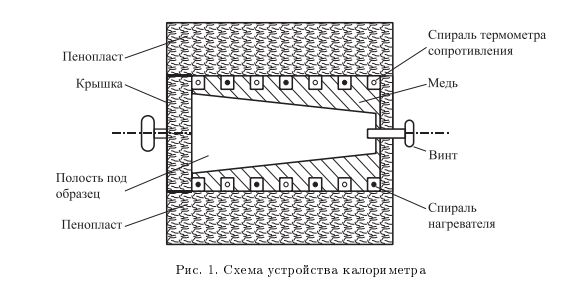
\includegraphics[width=0.9\linewidth]{kalorymetr.png}
\end{figure}
Итого, в этой работе нам нужно измерить 3 зависимости:
\begin{enumerate}
    \item \(R_{heat}(t)\) - зависимость показаний термометра сопротивления от температуры при постоянной мощности нагревателя.
    \item \(R_{cool}(t)\) - зависимость показаний термометра сопротивления от температуры при выключенном нагревателе.
    \item \(T_к(t)\) - фиксирование изменений температуры воздуха в течение эксперимента.
\end{enumerate}
\section{Методика эксперимента}
Я не буду приводить выкладки по получению формул (очень долго писать), но справедливо следующее:
\begin{equation}
    T(R) = 273 + \frac{R}{\alpha R_к} [1 + \alpha (T_к - 273)] - \frac{1}{\alpha}
\end{equation}

\begin{equation}
    T_{cool}(t) = (T_0 - T_к) e^{-\lambda t / C} + T_к
\end{equation}
\begin{equation}
    T_{heat}(t) = \frac{P}{\lambda}(1 - e^{-\lambda t / C}) + T_к\\
\end{equation}
Это был описан интегральный способ нахождения теплоемкостей.\\

Так же можно использовать другой способ. Возьмем точки на кривых нагревания и охлаждения при одинаковой темературе. Тогда обозначим за \(A = (\frac{\partial T}{\partial t})_{heat}\) и за \(B = (\frac{\partial T}{\partial t})_{cool}\). Тогда, используя два уравнения, которые мы получим через дифференцирование (6) и (7), получим следующее:
\begin{equation}
    \lambda = \frac{P}{(T - T_к)(1 - \frac{A}{B})}
\end{equation}

\begin{equation}
    C = \frac{P}{A - B}
\end{equation}

И так, нам предстоит изобразить на графике зависимость \(T_{cool}(t)\) в координатах \(y = ln(T_{cool} - T_к)/(T_0 - T_к)), x = t\), чтобы получить прямую с коэффициентом \(-\frac{\lambda}{C}\). Затем находим из уравнения (7) теплоемкость исслудуемой системы. Отсюда находим теплоемкости материалов. Эти результаты надо сравнить с результатами, полученными по дифференциальному методу, описанному выше.

\section{Обработка данных}
\subsection{Интегральный метод}
Итого, у меня получилось:
\begin{table}[h]
    \centering
    \begin{tabular}{|c|c|}
    \hline
         Система & \(\lambda/C, \ с^{-1}\) \\
    \hline
         Пустой калориметр      & \(0,380 \cdot 10^{-3}\) \\
         Калориметр + железо    & \(0,200 \cdot 10^{-3}\) \\
         Калориметр + аллюминий & \(0,195 \cdot 10^{-3}\) \\
    \hline
    \end{tabular}
\end{table}

Теперь найдем \(\lambda\). \(\lambda = (1 - e^{-\frac{\lambda t}{C}})\frac{P}{T_{heat} - T_к} = 0.17 \pm 0.02 \Rightarrow C_{кал} = 662 \pm 27 \frac{Дж}{К}\)
\\
Итого, получились следующие теплоемкости:
\begin{table}[h]
    \centering
    \begin{tabular}{|c|c|c|}
    \hline
         Материал & C, \(\frac{Дж}{К}\) & c, \(\frac{Дж}{К \cdot кг}\)  \\
    \hline
         Калориметр & 662,5 & - \\
         Железо     & 239,5 & 293,8 \\
         Аллюминий  & 116  &  395,9 \\
    \hline
    \end{tabular}
\end{table}
\subsection{Дифференциальный метод}
В этих таблицах находятся значения производных \(A \ и \ В\), а также значения теплоемкостей материалов.
\begin{table}[h]
    \begin{center}
        
    \begin{tabular}{|c|c|c|c|}
    \hline
        Производная & калориметр & калориметр + железо & калориметр + аллюминий \\
    \hline
         A &  0,007  & 0,004   & 0,006\\
    \hline
         B &  -0,002 & -0,001 & -0,002\\
    \hline
    \end{tabular}
    \end{center}
    \\
    \\
    \begin{center}
        \begin{tabular}{|c|c|c|}
        \hline
             материал   & C, \(\frac{Дж}{К}\) & c, \(\frac{Дж}{К \cdot кг}\)\\
        \hline
             калориметр &  589,1   & -\\
             железо     &  314,3   & 385,6\\
             аллюминий  &  168,1   & 571,7\\
        \hline    
    \end{tabular}  
    \end{center}
\end{table}
\newpage
\section{Графики}
\begin{figure}[h]
    \centering
    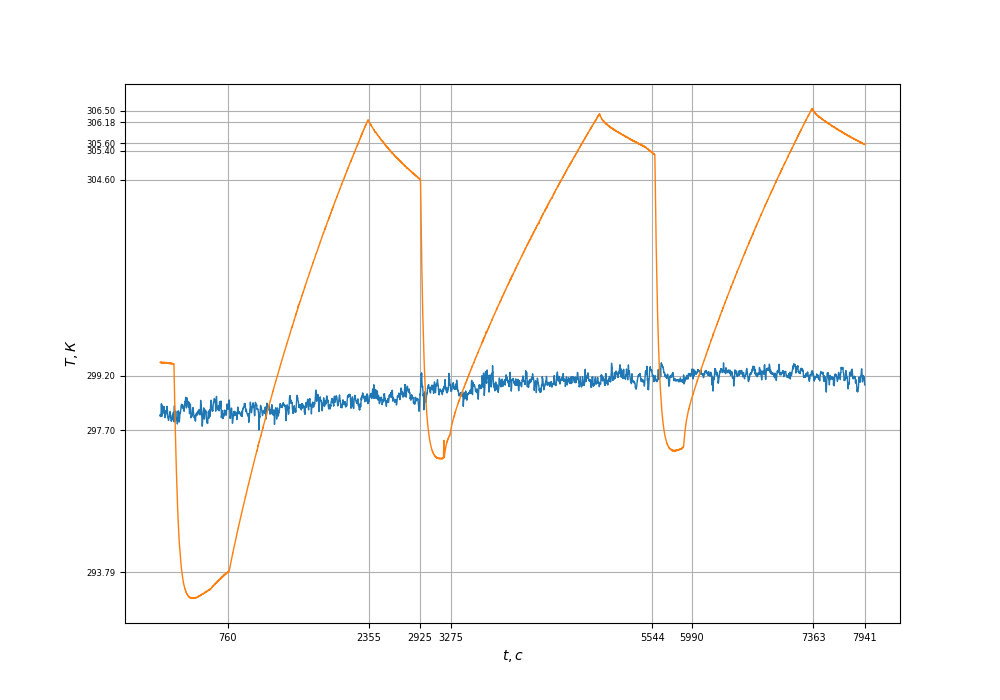
\includegraphics[width=1\linewidth]{plot_1.png}
\end{figure}
\begin{figure}[h]
    \centering
    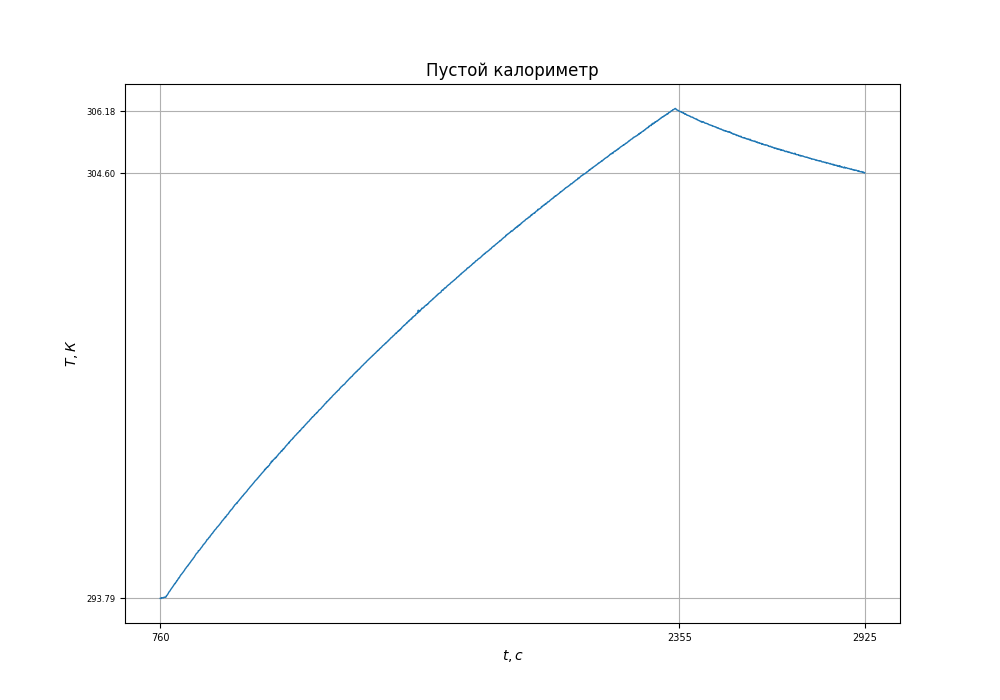
\includegraphics[width=1\linewidth]{plot_2.png}
\end{figure}
\begin{figure}[h]
    \centering
    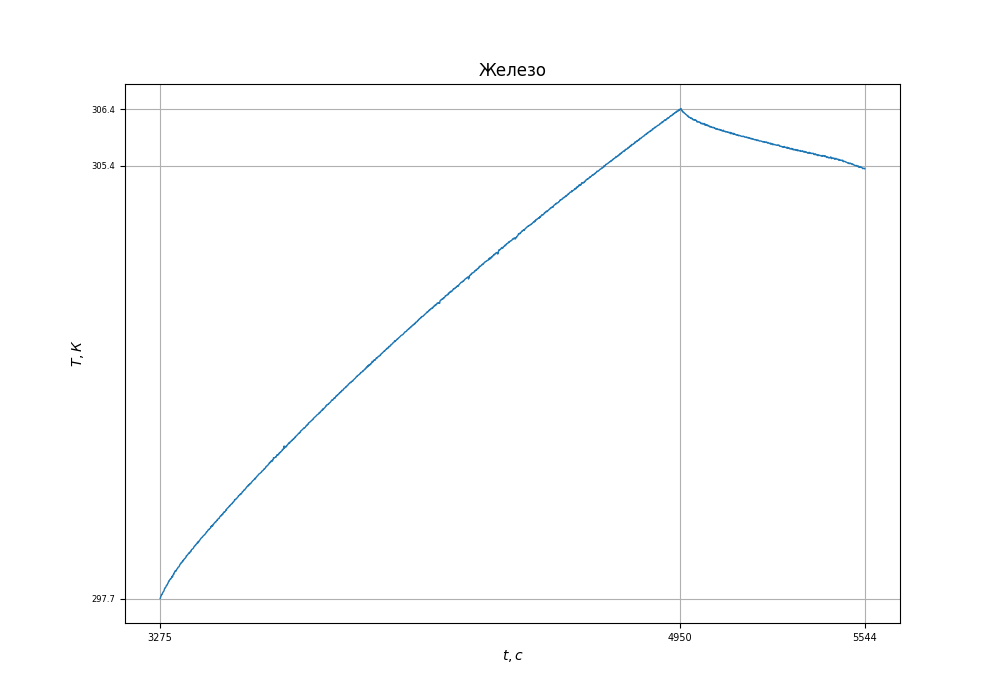
\includegraphics[width=1\linewidth]{plot_3.png}
\end{figure}
\begin{figure}[h]
    \centering
    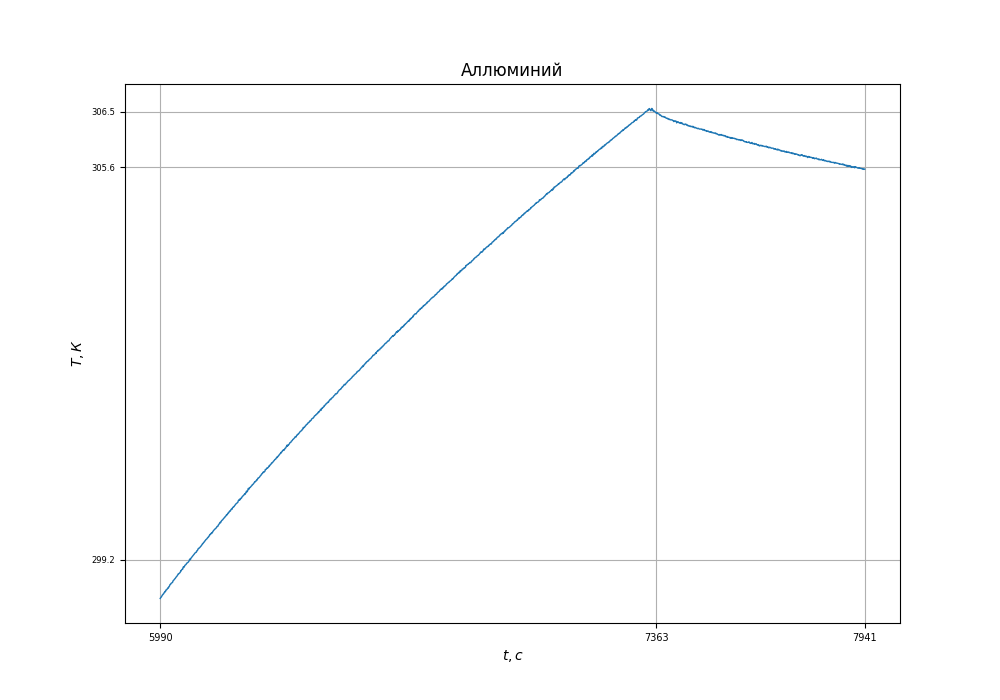
\includegraphics[width=1\linewidth]{plot_4.png}
\end{figure}
\begin{figure}[h]
    \centering
    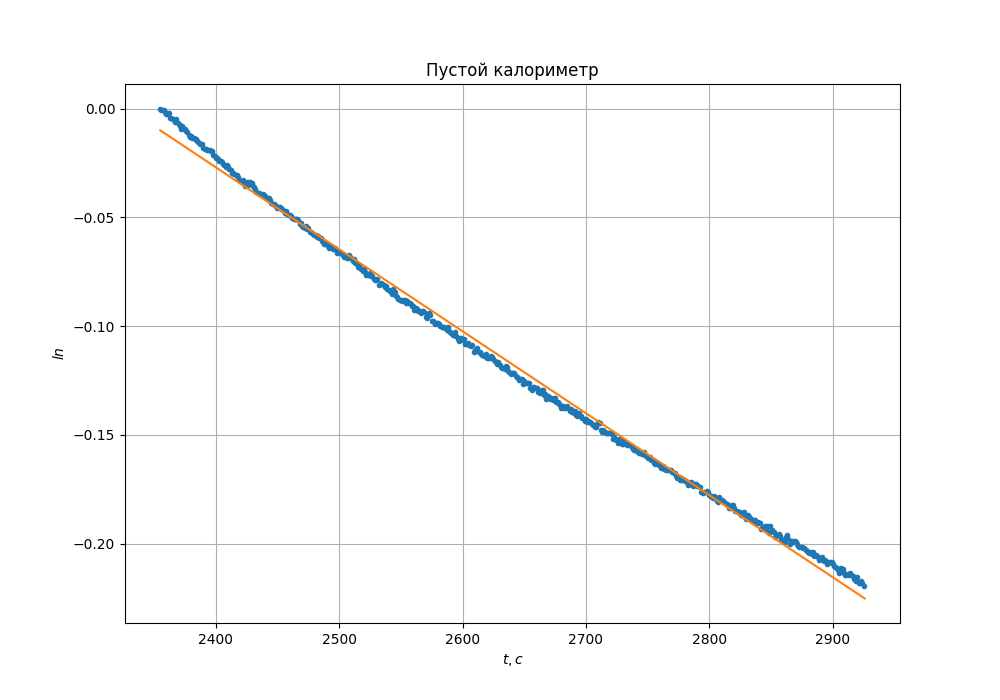
\includegraphics[width=1\linewidth]{ln_plot_1.png}
\end{figure}
\begin{figure}[h]
    \centering
    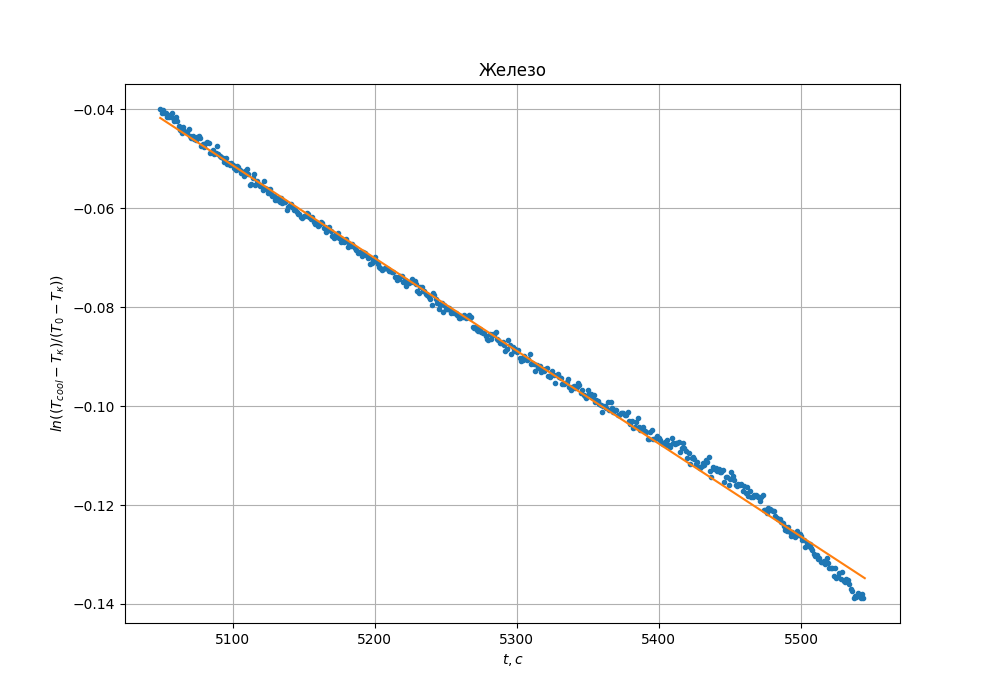
\includegraphics[width=1\linewidth]{ln_plot_2.png}
\end{figure}
\begin{figure}[h]
    \centering
    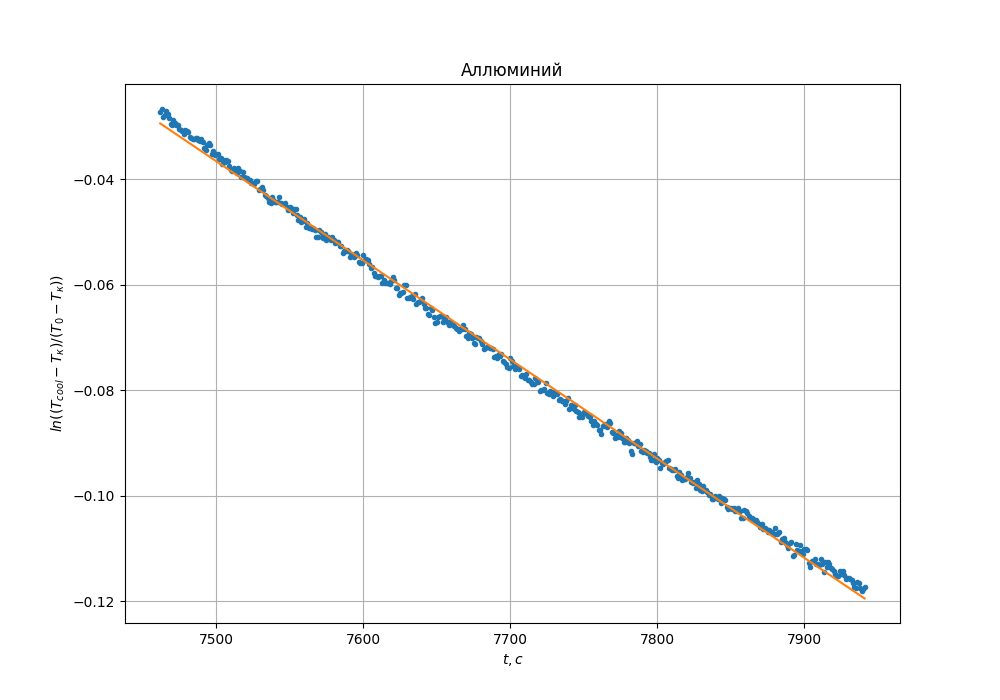
\includegraphics[width=1\linewidth]{ln_plot_3.png}
\end{figure}
\end{document}

\begin{table}[h]
    \centering
    
    \caption{Теплоемекости}
\end{table}
